\chapter{Chest X-Rays Automated Diagnosis}
\label{cha:third_chapter}

The goal of this chapter is to formally present the problem and introduce the dataset that we will use to train, evaluate and test the models that will be presented in the following chapter. In particular we want to give a description about the content of the dataset, its structure and also the pre-processing steps that have be done. 

\section{Problem Formulation}
\label{sec:problem_formulation}
The focus of this work is to build a system able to make accurate diagnoses of 14 different diseases analyzing an input image containing a chest x-ray. Formally, we have a dataset $D = \{(\mathbf{x}^{(\mathit{i})},\mathbf{y}^{(\mathit{i})}) ;\mathit{i}:1,...,N \}$ containing $N$ \acp{CXR}, where each image $\mathbf{x}^{(\mathit{i})}$ is associated with a set of label $\mathbf{y}^{(\mathit{i})} \in \{0,1\}^{14}$, where a value of 0 means that the corresponding disease is not present on the given input, while a value of 1, instead, means that it's present. We want our system to be able to predict, given a new instance $\mathbf{x}^{(\mathit{i})}$, the corresponding output  $\mathbf{y}^{(\mathit{i})}$. To be more specific, our system will carry out a value corresponding to the probability, for each pathology, to be present or not on a given \ac{CXR}. It is worth noting that this is not a multiclass classification problem, in which there is the assumption that a sample can be assigned to one and only one class, but it's a multilabel classification problem, in which a sample can be assigned to an arbitrary number of classes.

\vspace{3mm}
We also want our model to be able to produce a map highlighting the area of the image interested by the pathology and use it to automatically extract a bounding box around the disease region.

\section{Data Source}
\label{sec:data_source}
In our work we've decided to use CheXpert (\textbf{Che}st e\textbf{Xpert}), a large dataset released in 2019 by Stanford University for \ac{CXR} examination \cite{irvin2019chexpert}. 

\subsection{Content}
\label{sec:dataset_content}
The dataset is composed by 223,316 chest x-rays of 65,240 patients, collected by Stanford Hospital from October 2002 to July 2017.
The dataset is offered at two quality levels: the high quality one has a size of 439GB and the images are stored as 16-bit PNG, while the small version has a size of 11GB and stores the chest x-rays using a 8-bit PNG format. In this work, due to computational reasons, we have decided to use the small version.

\noindent Each image is annotated with 14 labels, that have been extracted from text radiology report using an automatic rule-based labeler. The labelling process can be divided in three different phases:
\begin{itemize}
    \item Mention Extraction: the \textit{Impression} section of the radiology report, which summarizes the key finding in the radiology study, is analyzed and a list of mentions is extracted. The extracted mentions are those that match a large list of phrases that has been manually created by multiple expert radiologist.
    \item Mention Classification: this phase aims at assigning each mention to a label among:
    \begin{itemize}
        \item Positive: the disease is confidently present
        \item Negative: the disease is confidently absent
        \item Uncertain: this value captures both the uncertainty in the radiologist diagnosis as well as the inherent ambiguity of the report.
    \end{itemize}
    \item Mention Aggregation: the last phase aggregates the classification of all the mentions in order to generate a label for all the 14 observations. Each label is assigned a positive (1), negative (0) or uncertain (\textit{u}) value if it has been explicitly mentioned in the report, while the (\textit{blank}) value is assigned to the unmentioned observations. 
\end{itemize}

\noindent The labeller has been tested by the Stanford Team against human labelled cases, showing that it is able to achieve very high perfomance.

\newpage
\noindent The labels have a hierarchical structure, that has been provided along with the dataset and can be seen in Figure \ref{fig:figure_3_1}. As we can see, for example, there is a dependency between Lung Opacity and Edema, meaning that an X-Ray presenting Edema must also contain a Lung Opacity (but the contrary must not necessarily be true). 

\begin{figure}[htbp!]
\centering
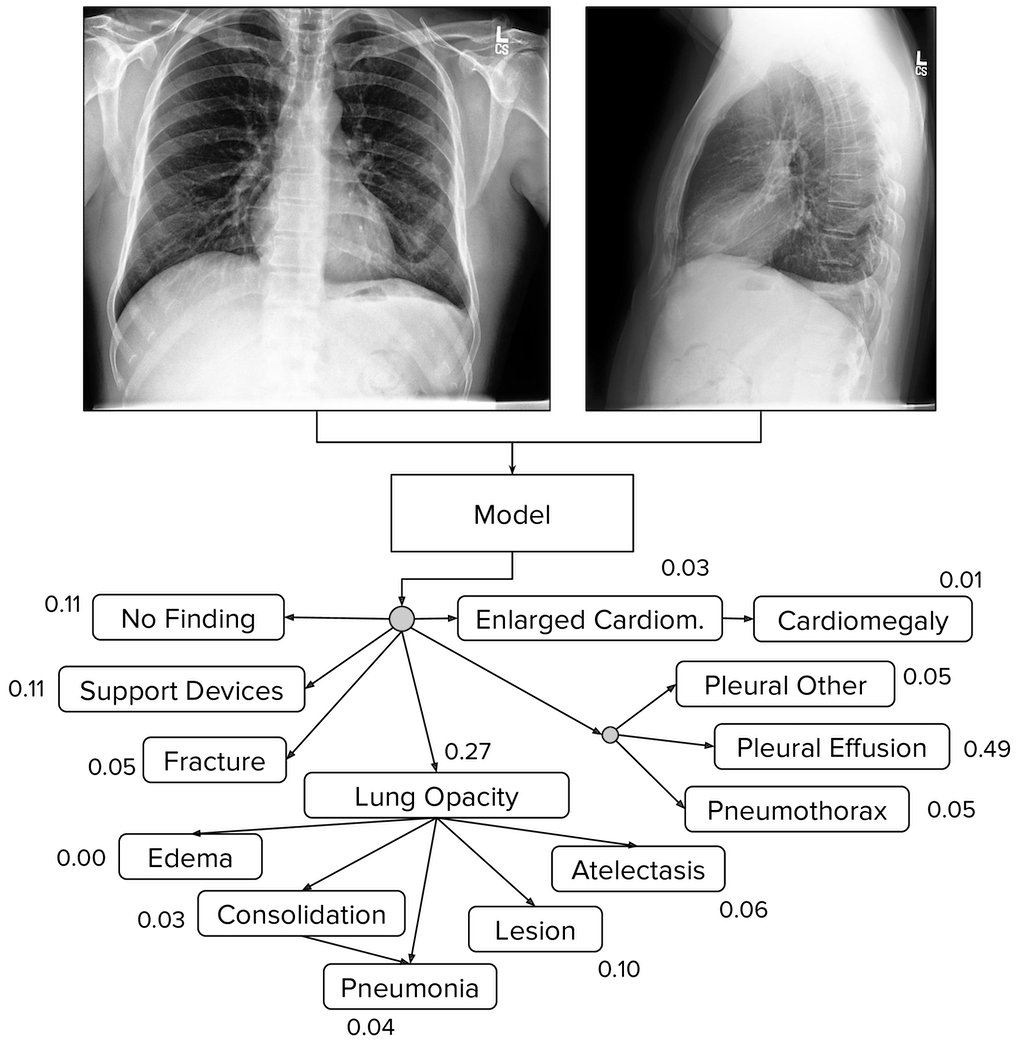
\includegraphics[scale=0.26]{Tesi/images/label_hierarchy}
\caption{Pathologies hierarchy}
\label{fig:figure_3_1}
\end{figure}

\noindent This additional information can be exploited in order to enhance the quality of the predictions.

\noindent Table \ref{table:table_1} gives a brief description of all the medical conditions that have been considered in the dataset. 

\newpage

\begin{table}[h!]

\centering

\begin{tabularx}{\textwidth}{|l|X|}
\hline
\textbf{Pathology Name}    & \textbf{Description}                                                                                 \\ 
\hline
No Finding                 & No pathology is assigned to a positive or uncertain label                                            \\ 
\hline
Enlarged Cardiomediastinum & Abnormal enlargement of the cardiomediastinal~silhouette                                             \\ 
\hline
Cardiomegaly               & Condition where the heart is enlarged.                                                                \\ 
\hline
Lung Lesion                & Damaged portion of a lung.                                                                           \\ 
\hline
Lung Opacity               & Area that attenuates x-ray beams, making the lung appearing more opaque than the surrounding region.  \\ 
\hline
Edema                      & Fluid accumulation in the tissue and air spaces of the lung.                                                                                                 \\ 
\hline
Consolidation              & Region of normally compressible lung tissue that has filled with liquid instead of air. The condition is marked by induration.                                                                                                    \\ 
\hline
Pneumonia                  & Pneumonia is an infection that inflames the air sacs in one or both lungs.                                                                                                      \\ 
\hline
Atelectasis                & Collapse or closure of a lung resulting in reduced or absent gas exchange.                                                                                                     \\ 
\hline
Pneumothorax               & Condition in which air accumulates in the pleural sac, causing it to expand and compress the underlying lung.                                                                                                     \\ 
\hline
Pleural Effusion           & Excess of fluid that accumulates in the pleural cavity.                                                                                                     \\ 
\hline
Pleural Other              & Other pleural disease                                                                                                      \\ 
\hline
Fracture                   & Partial or complete break in the continuity of a bone.                                                                                                      \\ 
\hline
Support Device             & Medical device aims at supporting or sustaining patient's life.                                                                                                      \\
\hline
\end{tabularx}
\caption{Definition of all the diseases considered in the dataset}
\label{table:table_1}
\end{table}



\subsection{Structure}
\label{sec:dataset_structure}
As mentioned in the previous section, the dataset contains 224,316 chest X-Rays extracted from 65,240 different patients. The details about the distribution of the different labels are reported in Table \ref{table:table_2}.


\begin{table}[h!]
\centering
\begin{tabular}{|l|l|l|l|} 
\hline
\textbf{Pathology}         &  \hfill \textbf{Positive (\%)}& \hfill \textbf{Uncertain (\%)}  & \hfill \textbf{Negative (\%)}   \\ 
\hline
No Finding        &    \hfill16627 (8.86)&      \hfill   0 (0.0)  & \hfill171014 (91.14)    \\\hline
Enlarged Cardiom. &    \hfill 9020 (4.81)&   \hfill 10148 (5.41)  & \hfill168473 (89.78)    \\\hline
Cardiomegaly      &  \hfill 23002 (12.26)&    \hfill 6597 (3.52)  & \hfill158042 (84.23)    \\\hline
Lung Lesion       &   \hfill  6856 (3.65)&   \hfill  1071 (0.57)  & \hfill179714 (95.78)    \\\hline
Lung Opacity      &  \hfill 92669 (49.39)&   \hfill  4341 (2.31)  & \hfill90631 (48.3)  \\\hline
Edema             &  \hfill 48905 (26.06)&   \hfill 11571 (6.17)  & \hfill127165 (67.77)    \\\hline
Consolidation     &  \hfill  12730 (6.78)&   \hfill23976 (12.78)  & \hfill150935 (80.44)    \\\hline
Pneumonia         &  \hfill   4576 (2.44)&   \hfill 15658 (8.34)  & \hfill167407 (89.22)    \\\hline
Atelectasis       & \hfill  29333 (15.63)&  \hfill 29377 (15.66)  & \hfill128931 (68.71)    \\\hline
Pneumothorax      & \hfill   17313 (9.23)&   \hfill  2663 (1.42)  & \hfill167665 (89.35)    \\\hline
Pleural Effusion  &  \hfill 75696 (40.34)&   \hfill  9419 (5.02)  & \hfill102526 (54.64)    \\\hline
Pleural Other     &  \hfill    2441 (1.3)&   \hfill  1771 (0.94)  & \hfill183429 (97.76)    \\\hline
Fracture          &  \hfill   7270 (3.87)&   \hfill   484 (0.26)  & \hfill179887 (95.87)    \\\hline
Support Device    &  \hfill 105831 (56.4)&   \hfill   898 (0.48)  &  \hfill80912 (43.12)   \\
\hline
\end{tabular}
\caption{Number of Positive, Uncertain and Negative labels for each disease}
\label{table:table_2}
\end{table}

The Stanford Team also provided a set of manually labeled images that can be used to assess the performance of the predictions. We additionally cut out a subset of data that will be used to tune the models' hyperparameters.
The dataset, moreover, contains two type of \acp{CXR}, the frontal-view and the lateral-view. Generally the latest one is performed as an adjunct to a frontal chest radiograph in cases where there is a diagnostic uncertainty. For this reason, the number of frontal images is much higher. The following table reports the numerical details about the dataset composition.

\vspace{5mm}

\begin{table}[h!]
\centering
\begin{tabular}{|l|l|l|} 
\hline
\textbf{Dataset}         &   \hfill \textbf{Frontal (\%)} &   \hfill \textbf{Lateral (\%)} \\
\hline
Training &    \hfill 189116 (84.56)   & \hfill 32387 (14.48) \\\hline
Validation &    \hfill 1911 (0.85)   & \hfill 0 (0.00)\\\hline
Test &    \hfill 202 (0.09) & \hfill 32 (0.01) \\

\hline
\end{tabular}
\caption{Dataset structure}
\label{table:table_3}
\end{table}


\section{Preprocessing}
\label{sec:preprocessing}
In this section we describe the preprocessing steps that have been done on the data before submitting them to the learning algorithms.

\vspace{5mm}

\noindent\textbf{Labels}

\vspace{5mm}

\noindent The author of the dataset provided, together with the images, two \textbf{.csv} files (one for the training set and one for the test set) mapping each \ac{CXR} with its own set of labels. Moreover, each image has additional information about the gender and the age of the patient that, however, in this work have not been considered. We also decided to focus our attention on the Frontal Chest X-Rays only, discarding the Lateral ones, that were available only for a relatively small amount of patients.

\noindent These are the steps we have done in order to clean the \textbf{.csv} files: 
\begin{itemize}
    \item The columns \textbf{"Sex"}, \textbf{"Age"}, \textbf{"Frontal/Lateral"}, \textbf{"AP/PA"} have been removed.
    \item The \textit{blank} values (i.e the unmentioned labels) have been assigned a value of 0.
    \item The uncertain labels, indicated with value -1, have been assigned a value that depends on the policy that have been used to deal with the uncertainties (we will give a more detailed explanation in section \ref{sec:uncertainty}).
\end{itemize}

\noindent The final \textbf{.csv} files were composed by a column containing the image reference and 14 additional columns, one for each disease, filled with a value indicating whether a particular pathology is present, not present or uncertain.


\vspace{5mm}

\noindent\textbf{Images}

\vspace{5mm}

\noindent Most of the images were affected by irrelevant noise such as text or irregular borders. Since these areas might affect the learning performance, we tried to solve the problem by removing them. So the \ac{CXR} images were first resized to $256 \times 256$ pixels and then a template matching algorithm has been applied in order to find a region of the image with size $224 \times 224$ containing a chest template. In many cases this approach successfully removed the irrelevant areas, as we can see in Figure \ref{fig:figure_3_2}. Moreover, the images have been converted to RGB in order to match the required input shape of the models and pixel values have been scaled in a range between 0 and 1. Finally, since the model we have used have been pre-trained on ImageNet \cite{imagenet}, we have normalized all the images with respect to mean and standard deviation of that dataset.

\vspace{5mm}


\begin{figure}[h!]
\centering
\begin{minipage}{.4\textwidth}
  \centering
  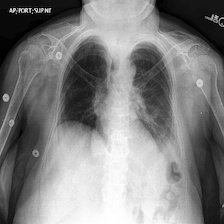
\includegraphics[width=5cm]{Tesi/images/img1}
  \caption*{Before}
\end{minipage}%
\begin{minipage}{.4\textwidth}
  \centering
  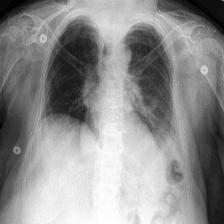
\includegraphics[width=5cm]{Tesi/images/img2}
  \caption*{After}

\end{minipage}
\caption{Comparison of \ac{CXR} before and after preprocessing}%
\label{fig:figure_3_2}
\end{figure}

\newpage
\noindent\textbf{Data Format}

\vspace{5mm}

\noindent When dealing with very large amount of data, using the proper data format could have a significant impact on the performance of the input pipeline and, consequently, on the training time of the model. In our work we have decided to use the TFRecord data format, that is Tensorflow’s own binary storage format.
TFRecord is extremely useful when dealing with large dataset that does not fit in RAM, because it allows to efficiently load and preprocess only the data that are required at the time. 
\noindent Each entry of our TFRecord file is composed by two elements: 
\begin{itemize}
    \item Image: serialized version of a \ac{CXR}
    \item Labels: vector of 14 elements, each one associated to a particular pathology.
\end{itemize}

\section{Related Works}
\label{sec:related_work}
Since it's introduction, there have been many works involving CheXpert. The first one has been released together with the dataset, in which the Stanford team developed a system able to classify and localize the different diseases exploiting a \ac{CNN}. Moreover, they explored different approaches to deal with the uncertain labels and, finally, compared their results with that of 3 radiologist, exceeding their score in most of the pathologies. 

\noindent The Stanford Machine Learning Group also set up a competition, called CheXpert \cite{chexpert_competition}, that allows people from all over the world to submit the result of their projects involving CheXpert. Among the different works, it worth mentioning that of Pham et al. \cite{pham2019interpreting}, that reached the first position on the competition. The key point of their work is the investigation of novel approaches to deal with the uncertain labels, the use of Ensemble, and the exploitation of the dependency among the diseases to improve the quality of the prediction.

\section{Summary}
\label{sec:summary_chapter_three}
In this chapter we have introduced the dataset that we will use in our work, presenting its composition and its structure. We have also also talked about the preprocessing steps that we have done before submitting the data to the training algorithms and, finally, we mentioned the related works that have been done involving the same dataset. In the next chapter we will dive into the core of this work, presenting a formal definition of the problem and the solution we have developed to solve it. 